\documentclass[UTF8]{ctexart}
\usepackage{listings} 
\usepackage{xcolor} 
\usepackage{caption}
\usepackage{palatino}
\usepackage{lipsum}
\usepackage{amsmath}  % 此处引入数学公式的包
\usepackage{amssymb}
\usepackage{graphicx} % 用于插入图片
\usepackage{subfigure}
\usepackage{float}
\usepackage{multirow}
\usepackage{caption}
\usepackage{indentfirst}
\usepackage{url}
\usepackage{hyperref}
\usepackage{pythonhighlight}
\usepackage{geometry}
\usepackage{longtable}
\usepackage{diagbox}
\usepackage{appendix}
\usepackage{array}
\usepackage{subfigure}
\usepackage{threeparttable}
\usepackage{graphicx}
\usepackage{booktabs}
\usepackage{fontspec}
\usepackage{titlesec}
\usepackage{hyperref}

\setmainfont{Times New Roman}
\renewcommand{\baselinestretch}{1.5}

\hypersetup{
colorlinks=true,
linkcolor=black,
citecolor=black
}
%页眉消失
\pagestyle{plain} 
%边界设置也就是,距离A4纸边框的距离
\geometry{a4paper,left=2.5cm,right=2.5cm,top=2.5cm,bottom=2.5cm}
%附录代码格式设置
\lstset{ 
  frame=tb,
  aboveskip=3mm,
  belowskip=3mm,
  showstringspaces=false,
  columns=flexible,
  framerule=1pt,
  rulecolor=\color{gray!35},
  backgroundcolor=\color{gray!5},
  basicstyle={\small\ttfamily},
  numbers=none,
  numberstyle=\tiny\color{gray},
  keywordstyle=\color{blue},
  commentstyle=\color{blue},
  stringstyle=\color{blue},
  breaklines=true,
  breakatwhitespace=true,
  tabsize=3,
}

\title{\textbf{珐玛-弗伦奇多因素模型和共同基金的收益研究} \vspace{-2.5em}}
\date{}
% \author{邓皓天}
\begin{document}
\maketitle
\centerline{邓皓天\quad2023310114}
\renewcommand{\abstractname}{\Large 摘要\\}
\begin{abstract}
  本文基于尤金·法玛和肯尼斯·弗伦奇提出的著名的三因素模型
  $R_{it}-\mathrm{RFR}_t=\alpha _i+\beta _1\left( R_{Mt}-\mathrm{RFR}_t \right) +\beta _2\mathrm{SMB}_t+\beta _3\mathrm{HML}_t+\varepsilon _{it}$,
  对共同基金Fidelity Magellan Fund(FMAGX)的历史收益率数据进行参数估计和模型验证。

  本文首先对各变量进行基础的描述性统计分析,
  而后对各变量水平时间序列进行单位根检验后,
  发现所有时间序列皆为平稳序列。
  分别对各解释变量和被解释变量进行格兰杰因果关系检验,
  发现其间皆存在双向影响。
  在进行多重共线性诊断后发现,
  各解释变量之家不存在严重的多重共线性问题,
  因此可进行进一步回归建模。

  经过最小二乘估计后得到的回归模型结果为
  $\text{FMAGX}_t-\mathrm{RFR}_t=-0.69+1.07\left( R_{Mt}-\mathrm{RFR}_t \right) -0.32\mathrm{SMB}_t-0.25\mathrm{HML}_t$,
  其调整后的决定系数高达0.82,
  说明模型的拟合效果良好,
  且布罗施-帕甘检验和怀特检验的结果皆说明模型不存在异方差问题,
  RESET检验结果说明模型不存在缺少高次项的设定偏误问题,
  可以认为模型的估计良好有效。

  同时,采用加入虚拟变量的方法验证
  模型定价因子的结构是否在疫情前后发生变化后,
  发现新冠疫情的冲击并未导致方程结构的改变;
  而改用
  共同基金Fidelity Low Priced Stock Fund(FLPSX)
  的历史收益率数据建立类似的方程,
  发现模型存在多重共线性和异方差问题。
  经过删除多余变量、加权最小二乘法估计和
  异方差稳健标准误法对上述问题进行修正后,
  发现仅有市场风险因子$R_{Mt}-\mathrm{RFR}_t$
  仍在模型中,
  说明针对不同类型的基金,定价模型结构可能发生改变。

  而对于模型估计系数的结果,
  可以发现市场风险因子对应系数为正,
  这与FMAGX主要投资于顺周期行业的事实相一致;
  SMB风险因子对应的系数为负,
  这与FMAGX主要投资于大盘股的事实一致;
  而HML风险因素对应的系数同样为负,
  这与其主要投资于“成长型”的公司的事实相符合。

  \textbf{关键字}:APT三因素模型\quad 共同基金收益率\quad 多元线性回归
\end{abstract}
\newpage
% \tableofcontents
% \newpage


\section{研究背景}

\subsection{三因素模型}

尤金·法玛和肯尼斯·弗伦奇提出的著名的三因素模型
可由如下回归公式表示:
\begin{equation}
  R_{it}-\mathrm{RFR}_t=\alpha _i+\beta _1\left( R_{Mt}-\mathrm{RFR}_t \right) +\beta _2\mathrm{SMB}_t+\beta _3\mathrm{HML}_t+\varepsilon _{it}
\end{equation}

其中,$R_{it}$是资产$i$在时间$t$的收益,
$\mathrm{RFR}_t$是在时间$t$的无风险利率,
$R_{Mt}$是市场在时间t的收益。

该回归方程中第1个风险因素$(R_{Mt}-\mathrm{RFR}_t)$代表资本资产定价模型中常用的市场因素;
第2个风险因素$\mathrm{SMB}$是计算市值小的股票组合的收益与市值大的股票组合的收益的差异,主要反映小公司效应;
第3个风险因素$\mathrm{HML}$是计算价值型股票组合的收益和成长型股票的收益之间的差异
(市场价值和账面价值比较低的股票归为价值型股票,反之则是成长型股票,模型中包含该因素是由于,历史上价值型股票的收益相对较高)。

如果市场风险因子对应的系数$\beta_1>0$,
则说明资产主要投资于顺周期行业,
反之则为逆周期行业;
而如果与公司规模相关的风险因素对应的系数$\beta_2>0$,
则说明资产主要投资于小盘股,
反之则为大盘股;
如果衡量“成长型”和“价值型”的风险因素对应的系数$\beta_3>0$,
则说明资产主要投资于“价值型”股票,
防止则为“成长型”股票。



而方程的截距项$\alpha_i$代表资产资产所获得的超额收益:
如果$\alpha_i>0$,则说明资产获得了一个高于根据其风险水平应该获得的收益,
如果$\alpha_i<0$,则代表资产获得了低于根据其风险水平应该获得的收益。
该指标即“詹姆森”$\alpha$,在共同基金的评价中广泛使用。

\subsection{定价资产选取}
本文选取Fidelity Magellan Fund(FMAGX)
历史收益率数据作为定价资产数据。
该基金始于1963年5月2日,
主要投资于共同基金、ETF、年金、存款证 、债券和其他投资工具等,
其基金规模高达11275.31亿元,
平均费用率仅为 0.40\%。
在彼得林奇管理的13年中,
年均收益率达29\%,
使业界极为震惊。
而如今的该基金的主旋律为“美国大型成长股”:
共73个不同的持股,
主要包括美国国大盘股和少量外国股票,
例如:Microsoft Corp、Apple Inc、Amazon.comInc、Meta Platforms Inc Class A、Alphabet Inc Class A等。
由于该基金主要投资于成长型股票和大盘股,
其投资风格可由下图表示:
\begin{figure}[H]
  \centering
  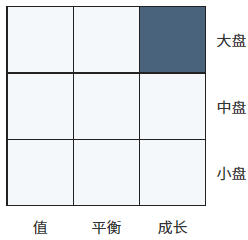
\includegraphics[scale=0.8]{pic/FMAGX投资风格.png}
  \caption{FMAGX投资风格}
\end{figure}



\subsection{数据来源}

法玛-弗伦奇的因素和无风险收益率数据来源于
\href{http://mba.tuck.dartmouth.edu/pages/faculty/ken.french/data_library.html}{弗伦奇的网站},
Fidelity Magellan Fund(FMAGX)和Fidelity Low Priced Stock Fund(FLPSX)的历史收益率数据来源于
\href{https://cn.investing.com/funds/fidelity-magellan-historical-data}{英为财情},
详细数据见附录。

\subsection{符号说明}

\setlength{\tabcolsep}{30mm}{
  \begin{table}[H]
    \centering
    \caption{符号说明}
    \resizebox{\textwidth}{!}{
      \begin{tabular}{cc}
        \toprule[1.5pt]
        符号     & 含义                                 \\ \midrule[0.75pt]
        FMAGX    & Fidelity Magellan Fund历史收益率     \\
        FLPSX    & Fidelity Low Priced Stock历史收益率  \\
        $R_M$       & 市场历史收益率                       \\
        RFR      & 历史无风险收益率                     \\
        SMB      & 市值大和市值小的股票组合的收益率差异 \\
        HML      & “价值型”和“成长型”股票收益率差异     \\
        $\alpha$ & 詹姆森-Alpha值                       \\
        $\beta$  & 风险因素对应贝塔系数                 \\ \bottomrule[1.5pt]
      \end{tabular}
    }
  \end{table}}

\section{描述性统计与平稳性检验}

\subsection{各变量描述性统计表}

\setlength{\tabcolsep}{8mm}{
  \begin{table}[H]
    \centering
    \caption{描述性统计}
    \resizebox{\textwidth}{!}{
      \begin{tabular}{ccccc}
        \toprule[1.5pt]
        Descriptive Stats & FMAGX-RFR & RM-RFR & SMB   & HML    \\ \midrule[0.75pt]
        Mean              & 0.93      & 1.36   & -0.04 & -0.65  \\
        Median            & 1.91      & 2.16   & -0.01 & -1.03  \\
        Maximum           & 12.94     & 13.65  & 7.00  & 7.41   \\
        Minimum           & -13.69    & -13.50 & -8.32 & -14.02 \\
        Std. Dev.         & 5.52      & 5.04   & 3.09  & 3.84   \\
        Skewness          & -0.54     & -0.49  & 0.16  & -0.30  \\
        Kurtosis          & 3.12      & 4.21   & 3.16  & 5.03   \\
        Jarque-Bera       & 2.46      & 5.11   & 0.26  & 9.55   \\
        Probability       & 0.29      & 0.08   & 0.88  & 0.01   \\
        Observations      & 51        & 51     & 51    & 51     \\ \bottomrule[1.5pt]
      \end{tabular}
    }
  \end{table}}



\subsection{平稳性检验}

\subsubsection{图示判断}
\begin{figure}[H]
  \centering
  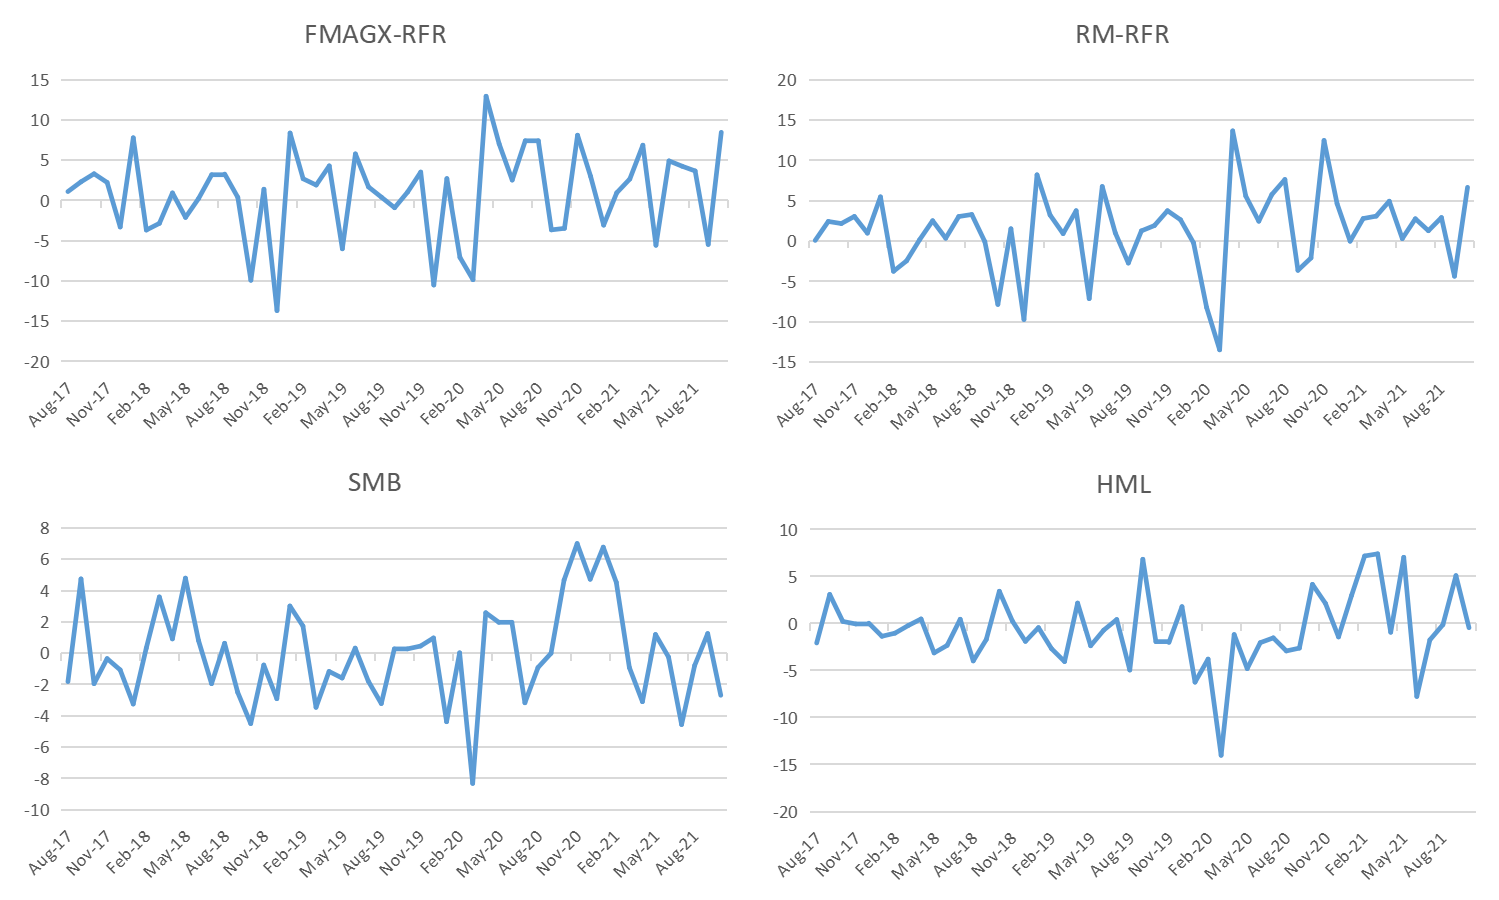
\includegraphics[scale=0.6]{./pic/时间序列平稳性.png}
  \caption{变量时间序列图}
\end{figure}

由上图可以看出,各变量的时间序列数据皆表现出围绕均值不断波动的过程,
因此可以推测各变量时间序列皆为平稳序列,不存在单位根。

\subsubsection{单位根检验}

(1)对FMAGX-RFR水平序列的检验

采用拉格朗日乘数法检验模型残差项的序列相关性,
对不引入滞后项的模型
$\Delta \text{FMAGX-RFR}_{t} = \alpha + \beta T +\delta \text{FMAGX-RFR}_{t-1}$。
首先进行普通最小二乘估计,
其D.W.统计量为2.02,
可以认为不存在序列相关性;
对1阶序列相关进行GB检验,
其LM(1)=0.49,对应的P值为0.48>0.05。
综上,即可认为随机干扰项不存在一阶序列相关。


同样,根据SIC准则确定的最大滞后项也为0阶
(即随机干扰项本身不存在序列相关,无需引入滞后项)。
由于后文中经过拉格朗日乘数法检验确定的滞后项阶数与通过SIC准则确定的结果完全一致,
故不再一一赘述,滞后阶数以SIC准则为准。
因此,ADF检验模型为:

模型3:$\Delta \text{FMAGX-RFR}_{t} = \alpha + \beta T +\delta \text{FMAGX-RFR}_{t-1}$

模型2:$\Delta \text{FMAGX-RFR}_{t} = \alpha + \delta  \text{FMAGX-RFR}_{t-1}$

模型1:$\Delta \text{FMAGX-RFR}_{t} = \delta \text{FMAGX-RFR}_{t-1}$


模型的原假设皆为$\text{H}_0:\delta=0$(即存在一单位根),
首先估计模型3,具体检验结果如下表所示:

\setlength{\tabcolsep}{8mm}{
  \begin{table}[H]
    \centering
    \caption{对FMAGX-RFR水平序列的ADF检验(同时包含趋势项和截距项)}
    \resizebox{\textwidth}{!}{
      \begin{tabular}{ccccc}
        \toprule[1.5pt]
        Variable      & Coefficient & Std. Error & t-Statistic & Test critical values (at 5 \% level) \\ \midrule[0.75pt]
        FMAGX-RFR(-1) & -1.21       & 0.14       & -8.38       & -3.50                                \\
        C             & -0.40       & 1.58       & -0.25       & 3.14                                 \\
        T             & 0.06        & 0.05       & 1.08        & 2.81                                 \\ \bottomrule[1.5pt]
      \end{tabular}
    }
  \end{table}}

从$\text{FMAGX-RFR}_{t-1}$的参数估计来看,
其$t_{\delta}$统计量的值为-8.38,
小于5\%显著性水平下的临界值-3.50(由ADF分布临界值表得),
因此,拒绝存在单位根的原假设;
而趋势项对应$t_{\beta}$统计量为1.08,
小于5\%显著性水平下的临界值2.81(同样由ADF分布临界值表得),
因此,不能拒绝不存在时间趋势项的原假设。
综合以上两项检验结果,需进一步估计和检验模型2。

对模型2($\Delta \text{FMAGX-RFR}_{t} = \alpha + \delta  \text{FMAGX-RFR}_{t-1}$)的检验结果如下表所示:
\setlength{\tabcolsep}{8mm}{
  \begin{table}[H]
    \centering
    \caption{对FMAGX-RFR水平序列的ADF检验(仅包含截距项)}
    \resizebox{\textwidth}{!}{
      \begin{tabular}{ccccc}
        \toprule[1.5pt]
        Variable      & Coefficient & Std. Error & t-Statistic & Test critical values (at 5\% level) \\ \midrule[0.75pt]
        FMAGX-RFR(-1) & -1.20       & 0.14       & -8.30       & -2.93                               \\
        C             & 1.08        & 0.79       & 1.37        & 2.56                                \\ \bottomrule[1.5pt]
      \end{tabular}
    }
  \end{table}}

从$\text{FMAGX-RFR}_{t-1}$的参数估计来看,
其$t_{\delta}$统计量的值为-8.30,
小于5\%显著性水平下的临界值-2.93(由ADF分布临界值表得),
因此,拒绝存在单位根的原假设;
而截距项对应$t_{\alpha}$统计量为1.37,
小于5\%显著性水平下的临界值2.56(同样由ADF分布临界值表得),
因此,不能拒绝不存在截距项的原假设。
综合以上两项检验结果,需进一步估计和检验模型1。


对模型1($\Delta \text{FMAGX-RFR}_{t} = \delta \text{FMAGX-RFR}_{t-1}$)的检验结果如下表所示:
\setlength{\tabcolsep}{8mm}{
  \begin{table}[H]
    \centering
    \caption{对FMAGX-RFR水平序列的ADF检验(不包含截距项和趋势项)}
    \resizebox{\textwidth}{!}{
      \begin{tabular}{ccccc}
        \toprule[1.5pt]
        Variable      & Coefficient & Std. Error & t-Statistic & Test critical values (at 5\% level) \\ \midrule[0.75pt]
        FMAGX-RFR(-1) & -1.17       & 0.14       & -8.12       & -1.95                               \\ \bottomrule[1.5pt]
      \end{tabular}
    }
  \end{table}}

从$\text{FMAGX-RFR}_{t-1}$的参数估计来看,
其$t_{\delta}$统计量的值为-8.12,
小于5\%显著性水平下的临界值-1.95(由ADF分布临界值表得),
因此,拒绝存在单位根的原假设。

综合上述检验结果,FMAGX-RFR序列不存在单位根,
说明FMAGX基金经过风险调整后的收益率序列
是一个0阶单整序列($\text{FMAGX-RFR} \sim I(0)$),
即该序列平稳。

$\ $

(2)对RM-RFR水平序列的检验

根据SIC准则确定的最大滞后项为0阶
(即本身不存在序列相关,无需引入滞后项),
因此,ADF检验模型为:

模型3:$\Delta \text{RM-RFR}_{t} = \alpha + \beta T +\delta \text{RM-RFR}_{t-1}$

模型2:$\Delta \text{RM-RFR}_{t} = \alpha + \delta  \text{RM-RFR}_{t-1}$

模型1:$\Delta \text{RM-RFR}_{t} = \delta \text{RM-RFR}_{t-1}$


模型的原假设皆为$\text{H}_0:\delta=0$(即存在一单位根),
首先估计模型3,具体检验结果如下表所示:

\setlength{\tabcolsep}{8mm}{
  \begin{table}[H]
    \centering
    \caption{对RM-RFR水平序列的ADF检验(同时包含趋势项和截距项)}
    \resizebox{\textwidth}{!}{
      \begin{tabular}{ccccc}
        \toprule[1.5pt]
        Variable   & Coefficient & Std. Error & t-Statistic & Test critical values (at 5\% level) \\ \midrule[0.75pt]
        RM-RFR(-1) & -1.11       & 0.15       & -7.59       & -3.50                               \\
        C          & 0.22        & 1.47       & 0.15        & 3.14                                \\
        T          & 0.05        & 0.05       & 1.01        & 2.81                                \\ \bottomrule[1.5pt]
      \end{tabular}
    }
  \end{table}}

从$\text{RM-RFR}_{t-1}$的参数估计来看,
其$t_{\delta}$统计量的值为-7.59,
小于5\%显著性水平下的临界值-3.50(由ADF分布临界值表得),
因此,拒绝存在单位根的原假设;
而趋势项对应$t_{\beta}$统计量为1.01,
小于5\%显著性水平下的临界值2.81(同样由ADF分布临界值表得),
因此,不能拒绝不存在时间趋势项的原假设。
综合以上两项检验结果,需进一步估计和检验模型2。

对模型2($\Delta \text{RM-RFR}_{t} = \alpha + \delta  \text{RM-RFR}_{t-1}$)的检验结果如下表所示:

\setlength{\tabcolsep}{8mm}{
  \begin{table}[H]
    \centering
    \caption{对RM-RFR水平序列的ADF检验(仅包含截距项)}
    \resizebox{\textwidth}{!}{
      \begin{tabular}{ccccc}
        \toprule[1.5pt]
        Variable   & Coefficient & Std. Error & t-Statistic & Test critical values (at 5\% level) \\ \midrule[0.75pt]
        RM-RFR(-1) & -1.09       & 0.15       & -7.52       & -2.93                               \\
        C          & 1.50        & 0.75       & 2.01        & 2.56                                \\ \bottomrule[1.5pt]
      \end{tabular}
    }
  \end{table}}

从$\text{RM-RFR}_{t-1}$的参数估计来看,
其$t_{\delta}$统计量的值为-7.52,
小于5\%显著性水平下的临界值-2.93(由ADF分布临界值表得),
因此,拒绝存在单位根的原假设;
而截距项对应$t_{\alpha}$统计量为2.01,
小于5\%显著性水平下的临界值2.56(同样由ADF分布临界值表得),
因此,不能拒绝不存在截距项的原假设。
综合以上两项检验结果,需进一步估计和检验模型1。

对模型1($\Delta \text{FMAGX-RFR}_{t} = \delta \text{FMAGX-RFR}_{t-1}$)的检验结果如下表所示:
\setlength{\tabcolsep}{8mm}{
  \begin{table}[H]
    \centering
    \caption{对RM-RFR水平序列的ADF检验(不包含截距项和趋势项)}
    \resizebox{\textwidth}{!}{
      \begin{tabular}{ccccc}
        \toprule[1.5pt]
        Variable   & Coefficient & Std. Error & t-Statistic & Test critical values (at 5\% level) \\ \midrule[0.75pt]
        RM-RFR(-1) & -1.02       & 0.15       & -7.04       & -1.95                               \\ \bottomrule[1.5pt]
      \end{tabular}
    }
  \end{table}}

从$\text{RM-RFR}_{t-1}$的参数估计来看,
其$t_{\delta}$统计量的值为-7.04,
小于5\%显著性水平下的临界值-1.95(由ADF分布临界值表得),
因此,拒绝存在单位根的原假设。

综合上述检验结果,RM-RFR序列不存在单位根,
说明市场经过风险调整后的收益率序列
是一个0阶单整序列($\text{RM-RFR} \sim I(0)$),
即该序列平稳。

$\ $

(3)对SMB水平序列的检验

根据SIC准则确定的最大滞后项为0阶
(即本身不存在序列相关,无需引入滞后项),
因此,ADF检验模型为:

模型3:$\Delta \text{SMB}_{t} = \alpha + \beta T +\delta \text{SMB}_{t-1}$

模型2:$\Delta \text{SMB}_{t} = \alpha + \delta  \text{SMB}_{t-1}$

模型1:$\Delta \text{SMB}_{t} = \delta \text{SMB}_{t-1}$


模型的原假设皆为$\text{H}_0:\delta=0$(即存在一单位根),
首先估计模型3,具体检验结果如下表所示:

\setlength{\tabcolsep}{8mm}{
  \begin{table}[H]
    \centering
    \caption{对SMB水平序列的ADF检验(同时包含趋势项和截距项)}
    \resizebox{\textwidth}{!}{
      \begin{tabular}{ccccc}
        \toprule[1.5pt]
        Variable & Coefficient & Std. Error & t-Statistic & Test critical values (at 5\% level) \\ \midrule[0.75pt]
        SMB(-1)  & -0.76       & 0.14       & -5.32       & -3.50                               \\
        C        & -0.19       & 0.89       & -0.21       & 3.14                                \\
        T        & 0.01        & 0.03       & 0.24        & 2.81                                \\ \bottomrule[1.5pt]
      \end{tabular}
    }
  \end{table}}

从$\text{SMB}_{t-1}$的参数估计来看,
其$t_{\delta}$统计量的值为-5.32,
小于5\%显著性水平下的临界值-3.50(由ADF分布临界值表得),
因此,拒绝存在单位根的原假设;
而趋势项对应$t_{\beta}$统计量为0.24,
小于5\%显著性水平下的临界值2.81(同样由ADF分布临界值表得),
因此,不能拒绝不存在时间趋势项的原假设。
综合以上两项检验结果,需进一步估计和检验模型2。

对模型2($\Delta \text{SMB}_{t} = \alpha + \delta  \text{SMB}_{t-1}$)的检验结果如下表所示:


\setlength{\tabcolsep}{8mm}{
  \begin{table}[H]
    \centering
    \caption{对SMB水平序列的ADF检验(仅包含截距项)}
    \resizebox{\textwidth}{!}{
      \begin{tabular}{ccccc}
        \toprule[1.5pt]
        Variable & Coefficient & Std. Error & t-Statistic & Test critical values (at 5\% level) \\ \midrule[0.75pt]
        SMB(-1)  & -0.76       & 0.14       & -5.38       & -2.93                               \\
        C        & -0.01       & 0.43       & -0.01       & 2.56                                \\ \bottomrule[1.5pt]
      \end{tabular}
    }
  \end{table}}

从$\text{SMB}_{t-1}$的参数估计来看,
其$t_{\delta}$统计量的值为-5.38,
小于5\%显著性水平下的临界值-2.93(由ADF分布临界值表得),
因此,拒绝存在单位根的原假设;
而截距项对应$t_{\alpha}$统计量为-0.01,
小于5\%显著性水平下的临界值2.56(同样由ADF分布临界值表得),
因此,不能拒绝不存在截距项的原假设。
综合以上两项检验结果,需进一步估计和检验模型1。

对模型1($\Delta \text{SMB}_{t} = \delta \text{SMB}_{t-1}$)的检验结果如下表所示:

\setlength{\tabcolsep}{8mm}{
  \begin{table}[H]
    \centering
    \caption{对SMB水平序列的ADF检验(不包含截距项和趋势项)}
    \resizebox{\textwidth}{!}{
      \begin{tabular}{ccccc}
        \toprule[1.5pt]
        Variable & Coefficient & Std. Error & t-Statistic & Test critical values (at 5\% level) \\ \midrule[0.75pt]
        SMB(-1)  & -0.76       & 0.14       & -5.43       & -1.95                               \\ \bottomrule[1.5pt]
      \end{tabular}
    }
  \end{table}}

从$\text{SMB}_{t-1}$的参数估计来看,
其$t_{\delta}$统计量的值为-7.04,
小于5\%显著性水平下的临界值-1.95(由ADF分布临界值表得),
因此,拒绝存在单位根的原假设。

综合上述检验结果,SMB序列不存在单位根,
说明小公司效应对应的风险因子序列
是一个0阶单整序列($\text{SMB} \sim I(0)$),
即该序列平稳。

$\ $

(4)对HML水平序列的检验

根据SIC准则确定的最大滞后项为0阶
(即本身不存在序列相关,无需引入滞后项),
因此,ADF检验模型为:

模型3:$\Delta \text{HML}_{t} = \alpha + \beta T +\delta \text{HML}_{t-1}$

模型2:$\Delta \text{HML}_{t} = \alpha + \delta  \text{HML}_{t-1}$

模型1:$\Delta \text{HML}_{t} = \delta \text{HML}_{t-1}$


模型的原假设皆为$\text{H}_0:\delta=0$(即存在一单位根),
首先估计模型3,具体检验结果如下表所示:


\setlength{\tabcolsep}{8mm}{
  \begin{table}[H]
    \centering
    \caption{对HML水平序列的ADF检验(同时包含趋势项和截距项)}
    \resizebox{\textwidth}{!}{
      \begin{tabular}{ccccc}
        \toprule[1.5pt]
        Variable & Coefficient & Std. Error & t-Statistic & Test critical values (at 5\% level) \\ \midrule[0.75pt]
        HML(-1)  & -0.94       & 0.15       & -6.46       & -3.50                               \\
        C        & -1.23       & 1.15       & -1.07       & 3.14                                \\
        T        & 0.03        & 0.04       & 0.65        & 2.81                                \\ \bottomrule[1.5pt]
      \end{tabular}
    }
  \end{table}}

从$\text{HML}_{t-1}$的参数估计来看,
其$t_{\delta}$统计量的值为-6.46,
小于5\%显著性水平下的临界值-3.50(由ADF分布临界值表得),
因此,拒绝存在单位根的原假设;
而趋势项对应$t_{\beta}$统计量为0.65,
小于5\%显著性水平下的临界值2.81(同样由ADF分布临界值表得),
因此,不能拒绝不存在时间趋势项的原假设。
综合以上两项检验结果,需进一步估计和检验模型2。

对模型2($\Delta \text{HML}_{t} = \alpha + \delta  \text{HML}_{t-1}$)的检验结果如下表所示:

\setlength{\tabcolsep}{8mm}{
  \begin{table}[H]
    \centering
    \caption{对HML水平序列的ADF检验(仅包含截距项)}
    \resizebox{\textwidth}{!}{
      \begin{tabular}{ccccc}
        \toprule[1.5pt]
        Variable & Coefficient & Std. Error & t-Statistic & Test critical values (at 5\% level) \\ \midrule[0.75pt]
        HML(-1)  & -0.93       & 0.14       & -6.46       & -2.93                               \\
        C        & -0.58       & 0.56       & -1.03       & 2.56                                \\ \bottomrule[1.5pt]
      \end{tabular}
    }
  \end{table}}

从$\text{HML}_{t-1}$的参数估计来看,
其$t_{\delta}$统计量的值为-6.46,
小于5\%显著性水平下的临界值-2.93(由ADF分布临界值表得),
因此,拒绝存在单位根的原假设;
而截距项对应$t_{\alpha}$统计量为-1.03,
小于5\%显著性水平下的临界值2.56(同样由ADF分布临界值表得),
因此,不能拒绝不存在截距项的原假设。
综合以上两项检验结果,需进一步估计和检验模型1。

对模型1($\Delta \text{HML}_{t} = \delta \text{HML}_{t-1}$)的检验结果如下表所示:

\setlength{\tabcolsep}{8mm}{
  \begin{table}[H]
    \centering
    \caption{对HML水平序列的ADF检验(不包含截距项和趋势项)}
    \resizebox{\textwidth}{!}{
      \begin{tabular}{ccccc}
        \toprule[1.5pt]
        Variable & Coefficient & Std. Error & t-Statistic & Test critical values (at 5\% level) \\ \midrule[0.75pt]
        HML(-1)  & -0.90       & 0.14       & -6.38       & -1.95                               \\ \bottomrule[1.5pt]
      \end{tabular}
    }
  \end{table}}

从$\text{HML}_{t-1}$的参数估计来看,
其$t_{\delta}$统计量的值为-7.04,
小于5\%显著性水平下的临界值-1.95(由ADF分布临界值表得),
因此,拒绝存在单位根的原假设。

综合上述检验结果,HML序列不存在单位根,
说明市场账面价值比对应的风险因子序列
是一个0阶单整序列($\text{HML} \sim I(0)$),
即该序列平稳。

$\ $


\section{模型建立}

\subsection{格兰杰因果关系检验}

对两变量$Y$与$X$,
格兰杰因果关系检验要求估计以下回归模型:
\begin{eqnarray}
  Y_{t}=\beta_{0}+\sum_{i=1}^{m} \beta_{i} Y_{t-i}+\sum_{i=1}^{m} \alpha_{i} X_{t-i}+\mu_{t}
  \\
  X_{t}=\delta_{0}+\sum_{i=1}^{m} \delta_{i} X_{t-i}+\sum_{i=1}^{m} \lambda_{i} Y_{t-i}+v_{t}
\end{eqnarray}

可能存在有四种检验结果:

(1)$X$对$Y$有单向影响,
表现为$X$各滞后项前的参数整体不为零,
而$Y$各滞后项前的参数整体为零;

(2)$Y$对$X$有单向影响,
表现为$Y$各滞后项前的参数整体不为零,
而$X$各滞后项前的参数整体为零;

(3)$Y$与$X$间存在双向影响,
表现为$X$各滞后项前的参数整体不为零,
同时$Y$各滞后项前的参数整体也不为零;

(4)$Y$与$X$是独立的,
表现为$X$各滞后项前的参数整体为零,
同时$Y$各滞后项前的参数整体也为零。

上述格兰杰因果关系检验可
通过受约束的$F$检验完成。
如针对$X$不是$Y$的格兰杰原因这一假设,
分别做包含与不包含$X$滞后项的回归,
记前者的残差平方和为$\mathrm{RSS}_\text{U}$,
后者的残差平方和为$\mathrm{RSS}_\text{R}$,
最后再计算$F$统计量的值:
\begin{eqnarray}
  F=\frac{\left(\operatorname{RSS}_{\mathrm{R}}-\mathrm{RSS}_{\mathrm{U}}\right) / m}{\mathrm{RSS}_{\mathrm{U}} /(n-k)}
\end{eqnarray}

\setlength{\tabcolsep}{18mm}{
  \begin{table}[H]
    \centering
    \caption{Pairwise Granger Causality Tests}
    \resizebox{\textwidth}{!}{
      \begin{tabular}{ccc}
        \toprule[1.5pt]
        Null Hypothesis                         & F-Statistic & Prob. \\ \midrule[0.75pt]
        RM-RFR does not Granger Cause FMAGX-RFR & 6.71        & 0.01  \\
        FMAGX-RFR does not Granger Cause RM-RFR & 1.67        & 0.44  \\
        SMB does not Granger Cause FMAGX-RFR    & 5.91        & 0.02  \\
        FMAGX-RFR does not Granger Cause SMB    & 1.62        & 0.42  \\
        HML does not Granger Cause FMAGX-RFR    & 7.09        & 0.01  \\
        FMAGX-RFR does not Granger Cause HML    & 0.38        & 0.93  \\ \bottomrule[1.5pt]
      \end{tabular}
    }
  \end{table}}

上表为检验模型取1阶滞后时的检验结果,
从$F$检验的P值来看,
模型中各解释变量对被解释变量单向因果关系检验的P值皆小于0.05,
可以认为各解释变量和被解释变量之间皆存在单向因果关系。

\subsection{多重共线性诊断}

\setlength{\tabcolsep}{12mm}{
  \begin{table}[H]
    \centering
    \caption{相关系数矩阵}
    \resizebox{\textwidth}{!}{
      \begin{tabular}{cccc}
        \toprule[1.5pt]
        Variable & RM-RFR & SMB  & HML  \\ \midrule[0.75pt]
        RM-RFR   & 1.00   & 0.39 & 0.20 \\
        SMB      & 0.39   & 1.00 & 0.44 \\
        HML      & 0.20   & 0.44 & 1.00 \\ \bottomrule[1.5pt]
      \end{tabular}
    }
  \end{table}}

由上表可以看出,
各解释变量之间的相关系数皆不高,
可以认为不存在高度相关性。


采用判定系数检验法,
以RM-RFR、SMB和HML分别为被解释变量,
其余为解释变量进行回归计算,
分别得到对应的判定系数$R_j^2$,
同时计算方差膨胀因子$\mathrm{VIF}=1/(1-R_j^2)$。



\setlength{\tabcolsep}{18mm}{
  \begin{table}[H]
    \centering
    \caption{方差膨胀因子}
    \resizebox{\textwidth}{!}{
      \begin{tabular}{ccc}
        \toprule[1.5pt]
        Dependent Variable & R-squared & VIF  \\ \midrule[0.75pt]
        RM-RFR             & 0.15      & 1.18 \\
        SMB                & 0.28      & 1.39 \\
        HML                & 0.19      & 1.24 \\ \bottomrule[1.5pt]
      \end{tabular}
    }
  \end{table}}

由上表可以看出,
各变量对应的R方较小,
方差膨胀因子都在1附近,
说明模型不存在严重的多重共线性问题。



\subsection{方程的显著性检验}

首先,尝试采用普通最小二乘法估计如下模型:
\begin{equation}
  \text{FMAGX}_t-\mathrm{RFR}_t=\beta_0+\beta_1\left( R_{Mt}-\mathrm{RFR}_t \right)+ \beta_2\mathrm{SMB}_t+\beta_3\mathrm{HML}_t + \mu_t
\end{equation}


对方程的显著性检验结果如下表所示:

\setlength{\tabcolsep}{12mm}{
  \begin{table}[H]
    \centering
    \caption{对方程的显著性检验}
    \resizebox{\textwidth}{!}{
      \begin{tabular}{cccc}
        \toprule[1.5pt]
        R-squared & Adjusted R-squared & F-statistic & Prob(F-statistic) \\ \midrule[0.75pt]
        0.83      & 0.82               & 78.93       & 0.00              \\ \bottomrule[1.5pt]
      \end{tabular}
    }
  \end{table}}


模型R方为0.83,
调整后的R方为0.82,
说明模型拟合效果良好;
F检验的P值为$0.00<0.05$,
表明模型的线性关系在5\%的显著性水平下显著成立。

\subsection{对系数的显著性检验}

接下来对方程中各变量的系数进行$t$检验:

\setlength{\tabcolsep}{8mm}{
  \begin{table}[H]
    \centering
    \caption{对系数的显著性检验}
    \resizebox{\textwidth}{!}{
      \begin{tabular}{ccccc}
        \toprule[1.5pt]
        Variable & Coefficient & Std. Error & t-Statistic & Prob. \\ \midrule[0.75pt]
        RM-RFR   & 1.07        & 0.07       & 15.13       & 0.00  \\
        SMB      & -0.32       & 0.13       & -2.58       & 0.01  \\
        HML      & -0.25       & 0.09       & -2.59       & 0.01  \\
        C        & -0.69       & 0.34       & -2.00       & 0.05  \\ \bottomrule[1.5pt]
      \end{tabular}
    }
  \end{table}}

根据上表,在5\%显著性水平下
各解释变量的$t$检验皆显著(P值均小于0.05)。
据此,可初步建立回归方程如下:
\begin{equation}
  \text{FMAGX}_t-\mathrm{RFR}_t=-0.69+1.07\left( R_{Mt}-\mathrm{RFR}_t \right) -0.32\mathrm{SMB}_t-0.25\mathrm{HML}_t
\end{equation}





\section{计量经济学检验}





\subsection{异方差检验}

由于最小二乘估计需满足同方差性假定,
否则估计会产生一系列不良后果,因此
分别采用布罗施-帕甘检验和怀特检验对模型异方差性进行检验。

\subsubsection{布罗施-帕甘检验(B-P检验)}

原线性模型为:
\begin{equation}
  \text{FMAGX}_t-\mathrm{RFR}_t=\beta_0+\beta_1\left( R_{Mt}-\mathrm{RFR}_t \right)+ \beta_2\mathrm{SMB}_t+\beta_3\mathrm{HML}_t + \mu_t
\end{equation}

使用普通最小二乘估计得到的残差项$e_t$
代替无法观测的$\mu_t$,
建立辅助回归:
\begin{equation}
  e_t^2 = \delta_0+\delta_1\left(R_{Mt}-\mathrm{RFR}_t\right)+\delta_2\mathrm{SMB}_t+\delta_3\mathrm{HML}_t + \varepsilon_t
\end{equation}

检验联合假设:
\begin{equation}
  \mathrm{H_0}:\delta_1=\delta_2=\delta_3=0
\end{equation}

通过以上述假设为约束条件的受约束$F$检验
或拉格朗日乘数(LM)检验即可对联合假设进行检验。
记辅助回归式的可决定系数为$R_{e^2}^2$,则
\begin{equation}
  F=\frac{R_{e^{2}}^{2} / k}{\left(1-R_{e^{2}}^{2}\right) /(T-k-1)} \sim F(k,T-k-1)
\end{equation}

\begin{equation}
  \mathrm{LM}=T \cdot R_{e^{2}}^{2}\ \dot \sim\ \chi^{2}(k)
\end{equation}

下表为布罗施-帕甘检验的结果:

\setlength{\tabcolsep}{30mm}{
  \begin{table}[H]
    \centering
    \caption{B-P检验}
    \resizebox{\textwidth}{!}{
      \begin{tabular}{cc}
        \toprule[1.5pt]
        Heteroskedasticity Test & Breusch-Pagan-Godfrey \\ \midrule[0.75pt]
        R-squared               & 0.02                  \\
        F-statistic             & 0.26                  \\
        Obs*R-squared           & 0.84                  \\
        Prob. F(3,47)           & 0.85                  \\
        Prob. Chi-Square(3)     & 0.84                  \\ \bottomrule[1.5pt]
      \end{tabular}
    }
  \end{table}}

表中的R-squared即为$R_{e^2}^{2}$,
其保留6位小数后的值为0.016421。
据此,即可分别计算$F$统计量的值和$\mathrm{LM}$统计量的值:


\begin{equation}
  F=\frac{R_{e^2}^{2}/k}{\left( 1-R_{e^2}^{2} \right) /(T-k-1)}=\frac{0.016421/3}{\left( 1-0.016421 \right) /\left( 51-3-1 \right)}=0.26
\end{equation}

\begin{equation}
  \mathrm{LM}=T \cdot R_{e^{2}}^{2} = 51\times 0.016421 = 0.84
\end{equation}

在5\%显著性水平下,
自由度为(3,47)的$F$分布的临界值为$F_{0.05}(3,47)=2.80$,
自由度为3的$\chi^2$分布的临界值为$\chi^2_{0.05}=7.81$。
因此,可以在5\%显著性水平下
接受原模型随机干扰项的方差相同的假设。


\subsubsection{怀特检验(White检验)}

考察$\mu^2$是部分或全部解释变量函数中包含非线性关系的形式,
原模型为:
\begin{equation}
  \text{FMAGX}_t-\mathrm{RFR}_t=\beta_0+\beta_1\left( R_{Mt}-\mathrm{RFR}_t \right)+ \beta_2\mathrm{SMB}_t+\beta_3\mathrm{HML}_t + \mu_t
\end{equation}

使用普通最小二乘估计得到的残差项的平方$e_t^2$做如下辅助回归:
\begin{equation}
  \begin{array}{l}
    e_{t}^{2} = \delta _0+\delta _1\left( R_{Mt}-\mathrm{RFR}_t \right) +\delta _2\mathrm{SMB}_t+\delta _3\mathrm{HML}_t                                             \\
    +\delta _4\left( R_{Mt}-\mathrm{RFR}_t \right) ^2+\delta _5\mathrm{SMB}_{t}^{2}+\delta _6\mathrm{HML}_{t}^{2}                                                    \\
    +\delta _7\left( R_{Mt}-\mathrm{RFR}_t \right) \mathrm{SMB}_t+\delta _8\left( R_{Mt}-\mathrm{RFR}_t \right) \mathrm{HML}_t+\delta _9\mathrm{SMB}_t\mathrm{HML}_t \\
  \end{array}
\end{equation}

待检验的同方差性假设为:
\begin{equation}
  \mathrm{H_0}:\delta_1=\delta_2=\cdots=\delta_9=0
\end{equation}

类似于B-P检验,
通过以上述假设为约束条件的受约束$F$检验
或拉格朗日乘数(LM)检验即可对联合假设进行检验。
记辅助回归式的可决定系数为$R_{e^2}^2$,则
\begin{equation}
  F=\frac{R_{e^{2}}^{2} / k}{\left(1-R_{e^{2}}^{2}\right) /(T-k-1)} \sim F(k,T-k-1)
\end{equation}

\begin{equation}
  \mathrm{LM}=T \cdot R_{e^{2}}^{2}\ \dot \sim\ \chi^{2}(k)
\end{equation}

下表为怀特检验的结果:

\setlength{\tabcolsep}{30mm}{
  \begin{table}[H]
    \centering
    \caption{White检验}
    \resizebox{\textwidth}{!}{
      \begin{tabular}{cc}
        \toprule[1.5pt]
        Heteroskedasticity Test & White \\ \midrule[0.75pt]
        R-squared               & 0.06  \\
        F-statistic             & 0.29  \\
        Obs*R-squared           & 3.10  \\
        Prob. F(9,41)           & 0.97  \\
        Prob. Chi-Square(9)     & 0.96  \\ \bottomrule[1.5pt]
      \end{tabular}
    }
  \end{table}}

表中的R-squared即为$R_{e^2}^{2}$,
其保留6位小数后的值为0.060777。
据此,即可分别计算$F$统计量的值和$\mathrm{LM}$统计量的值:




\begin{equation}
  F=\frac{R_{e^2}^{2}/k}{\left( 1-R_{e^2}^{2} \right) /(T-k-1)}=\frac{0.060777/9}{\left( 1-0.060777 \right) /\left( 51-9-1 \right)}=0.29
\end{equation}

\begin{equation}
  \mathrm{LM}=T \cdot R_{e^{2}}^{2} = 51\times 0.060777 = 3.10
\end{equation}

在5\%显著性水平下,
自由度为(9,41)的$F$分布的临界值为$F_{0.05}(3,47)=2.12$,
自由度为9的$\chi^2$分布的临界值为$\chi^2_{0.05}=16.92$。
因此,可以在5\%显著性水平下
接受原模型随机干扰项的方差相同的假设。

综上所述,
可以认为回归模型
$\text{FMAGX}_t-\mathrm{RFR}_t=-0.69+1.07\left( R_{Mt}-\mathrm{RFR}_t \right) -0.32\mathrm{SMB}_t-0.25\mathrm{HML}_t$
不存在异方差性问题。



\subsection{模型设定偏误}


\subsubsection{对是否含有无关变量的检验}

\setlength{\tabcolsep}{8mm}{
  \begin{table}[H]
    \centering
    \caption{对系数的显著性检验}
    \resizebox{\textwidth}{!}{
      \begin{tabular}{ccccc}
        \toprule[1.5pt]
        Variable & Coefficient & Std. Error & t-Statistic & Prob. \\ \midrule[0.75pt]
        RM-RFR   & 1.07        & 0.07       & 15.13       & 0.00  \\
        SMB      & -0.32       & 0.13       & -2.58       & 0.01  \\
        HML      & -0.25       & 0.09       & -2.59       & 0.01  \\
        C        & -0.69       & 0.34       & -2.00       & 0.05  \\ \bottomrule[1.5pt]
      \end{tabular}
    }
  \end{table}}

根据对方程中各解释变量系数的$t$检验的结果(P值全部小于0.05),
可以判断模型中三个解释变量(RM-RFR、SMB和HML)
皆非无关变量。


\subsubsection{对一般性设定偏误的检验}

考察原模型$\text{FMAGX}_t-\mathrm{RFR}_t=\beta_0+\beta_1\left( R_{Mt}-\mathrm{RFR}_t \right)+ \beta_2\mathrm{SMB}_t+\beta_3\mathrm{HML}_t + \mu_t$
是否存在遗漏了高次项的情况,
采用RESET检验法,
首先对原模型进行估计得:
\begin{equation}
  \text{FMAGX}_t-\mathrm{RFR}_t=\hat{Y}_t=\hat\beta_0+\hat\beta_1\left( R_{Mt}-\mathrm{RFR}_t \right)+ \hat\beta_2\mathrm{SMB}_t+\hat\beta_3\mathrm{HML}_t
\end{equation}

将估计出的$\hat{Y}_t$的高次幂引入模型,
通过$t$检验判断是否应该引入“非线性”因素。
待估计的模型如下:
\begin{equation}
  \text{FMAGX}_t-\mathrm{RFR}_t=\beta_0+\beta_1\left( R_{Mt}-\mathrm{RFR}_t \right)+ \beta_2\mathrm{SMB}_t+\beta_3\mathrm{HML}_t+\gamma_1\hat{Y}_t^2+\gamma_2\hat{Y}_t^3
\end{equation}


\setlength{\tabcolsep}{8mm}{
  \begin{table}[H]
    \centering
    \caption{RESET检验}
    \resizebox{\textwidth}{!}{
      \begin{tabular}{ccccc}
        \toprule[1.5pt]
        Variable    & Coefficient & Std. Error & t-Statistic & Prob. \\ \midrule[0.75pt]
        RM-RFR      & 0.98        & 0.15       & 6.67        & 0.00  \\
        SMB         & -0.33       & 0.13       & -2.56       & 0.01  \\
        HML         & -0.25       & 0.10       & -2.52       & 0.02  \\
        C           & -0.37       & 0.51       & -0.72       & 0.47  \\
        $\hat{Y}^2$ & -0.01       & 0.01       & -0.80       & 0.43  \\
        $\hat{Y}^3$ & 0.00        & 0.00       & 0.72        & 0.47  \\ \bottomrule[1.5pt]
      \end{tabular}
    }
  \end{table}}

从上表可以看出加入的高次幂项$t$检验皆不显著,
说明模型不应纳入非线性因素。
该模型的可决系数$R^2_{U}=0.837023$,
而原模型的可决系数$R^2_{R}=0.834391$。
据此可计算$F$统计量:
\begin{eqnarray}
  F=\frac{\left( R_{U}^{2}-R_{R}^{2} \right) /q}{\left( 1-R_{U}^{2} \right) /(T-(k+q+1))}=\frac{\left( 0.837023-0.834391 \right) /2}{\left( 1-0.837023 \right) /\left( 51-\left( 3+2+1 \right) \right)}=0.36
\end{eqnarray}

而5\%显著性水平下,
自由度为$(2,45)$的F分布的临界值为3.2,
不能拒绝联合假设$H_0:\gamma_1=\gamma_2=0$,
不应引入非线性项。

综上,可以认为原模型不存在模型设定偏误。




\subsection{疫情影响}

通过引入加法和乘法形式的虚拟变量,
检验新冠疫情前后,
模型的结构是否发生变化。
估计模型如下:
\begin{equation}
  \begin{matrix}
    \mathrm{FMAGX}_t-\mathrm{RFR}_t=\beta _0+\gamma _0D_t+\beta _1\left( R_{Mt}-\mathrm{RFR}_t \right) +\beta _2\mathrm{SMB}_t+\beta _3\mathrm{HML}_t \\
    \quad\quad\quad+\gamma _1D_t\left( R_{Mt}-\mathrm{RFR}_t \right) +\gamma _2D_t\mathrm{SMB}_t+\gamma _3D_t\mathrm{HML}_t                           \\
  \end{matrix}
\end{equation}

其中,$D$为引入的虚拟变量,
发生疫情前取值1,
发生疫情后取值2:
\begin{equation}
  D=\begin{cases}
    1,\text{发生疫情前} \\
    0,\text{发生疫情后} \\
  \end{cases}
\end{equation}

\setlength{\tabcolsep}{8mm}{
  \begin{table}[H]
    \centering
    \caption{引入虚拟变量的回归结果}
    \resizebox{\textwidth}{!}{
      \begin{tabular}{ccccc}
        \toprule[1.5pt]
        Variable   & Coefficient & Std. Error & t-Statistic & Prob. \\ \midrule[0.75pt]
        C          & -0.08       & 0.56       & -0.14       & 0.89  \\
        D          & -1.07       & 0.73       & -1.47       & 0.15  \\
        RM-RFR     & 1.03        & 0.09       & 11.31       & 0.00  \\
        SMB        & -0.35       & 0.17       & -2.05       & 0.05  \\
        HML        & -0.19       & 0.12       & -1.57       & 0.12  \\
        D×(RM-RFR) & 0.09        & 0.15       & 0.59        & 0.56  \\
        D×SMB      & -0.01       & 0.26       & -0.05       & 0.96  \\
        D×HML      & -0.14       & 0.21       & -0.65       & 0.52  \\ \bottomrule[1.5pt]
      \end{tabular}
    }
  \end{table}}

在5\%显著性水平下,无法拒绝各$\gamma$等于0的假设,
即各$\gamma$对应的变量是统计不显著的。
其中$t$统计量的绝对值最小的项对应变量为D×SMB,
故删掉该项后,
重新进行OLS估计新模型。
同样,所得结果中各$\gamma$对应的变量是统计不显著的,
$t$统计量的绝对值最小的项对应变量为D×(RM-RFR),
删除该项后再次重新进行OLS估计,
同理,直到删除全部$\gamma$对应的变量为止,
发现全部不显著。
综上,即可认为
疫情前后APT三因子定价模型的结构未发生变化。



\subsection{模型针对不同基金收益率定价的适用性}

以Fidelity Low Priced Stock(FLPSX)的历史收益率数据
对模型的适用性进行验证。
该基金成立于1989年12月27日,
主要投资于中盘股和价值型股票,
其投资组合主要由股票组成,
持有数百只股票和相当一部分国际股票:
1989年主要投资中小型股票和混合型股票,
在2003年转向小型混合型股票,
2005年转向中型混合型股票,
2014年转向中盘价值型股票,
投资于微软和甲骨文等大公司,
成功提升了基金的收益率。
而目前的重点则放在中盘价值的股票上。

\subsubsection{平稳性检验}

由于不同基金收益率定价因子相同,
前文中以对各因子时间序列数据平稳性进行过检验,
故此处不在赘述,
仅对FLPSX-RFR时间序列进行检验。

根据SIC准则确定的最大滞后项为0阶
(即本身不存在序列相关,无需引入滞后项),
因此,ADF检验模型为:

模型3:$\Delta \text{FLPSX-RFR}_{t} = \alpha + \beta T +\delta \text{FLPSX-RFR}_{t-1}$

模型2:$\Delta \text{FLPSX-RFR}_{t} = \alpha + \delta  \text{FLPSX-RFR}_{t-1}$

模型1:$\Delta \text{FLPSX-RFR}_{t} = \delta \text{FLPSX-RFR}_{t-1}$


模型的原假设皆为$\text{H}_0:\delta=0$(即存在一单位根),
首先估计模型3,具体检验结果如下表所示:




\setlength{\tabcolsep}{8mm}{
  \begin{table}[H]
    \centering
    \caption{对FLPSX-RFR水平序列的ADF检验(同时包含趋势项和截距项)}
    \resizebox{\textwidth}{!}{
      \begin{tabular}{ccccc}
        \toprule[1.5pt]
        Variable      & Coefficient & Std. Error & t-Statistic & Test critical values (at 5\% level) \\ \midrule[0.75pt]
        FLPSX-RFR(-1) & -1.03       & 0.15       & -7.08       & -3.50                               \\
        C             & -1.21       & 1.68       & -0.72       & 3.14                                \\
        T             & 0.05        & 0.06       & 0.86        & 2.81                                \\ \bottomrule[1.5pt]
      \end{tabular}
    }
  \end{table}}

从$\text{FLPSX-RFR}_{t-1}$的参数估计来看,
其$t_{\delta}$统计量的值为-7.08,
小于5\%显著性水平下的临界值-3.50(由ADF分布临界值表得),
因此,拒绝存在单位根的原假设;
而趋势项对应$t_{\beta}$统计量为-0.72,
小于5\%显著性水平下的临界值2.81(同样由ADF分布临界值表得),
因此,不能拒绝不存在时间趋势项的原假设。
综合以上两项检验结果,需进一步估计和检验模型2。

对模型2($\Delta \text{FLPSX-RFR}_{t} = \alpha + \delta  \text{FLPSX-RFR}_{t-1}$)的检验结果如下表所示:


\setlength{\tabcolsep}{8mm}{
  \begin{table}[H]
    \centering
    \caption{对FLPSX-RFR水平序列的ADF检验(仅包含截距项)}
    \resizebox{\textwidth}{!}{
      \begin{tabular}{ccccc}
        \toprule[1.5pt]
        Variable      & Coefficient & Std. Error & t-Statistic & Test critical values (at 5\% level) \\ \midrule[0.75pt]
        FLPSX-RFR(-1) & -1.02       & 0.14       & -7.05       & -2.93                               \\
        C             & 0.06        & 0.82       & 0.07        & 2.56                                \\ \bottomrule[1.5pt]
      \end{tabular}
    }
  \end{table}}

从$\text{FLPSX-RFR}_{t-1}$的参数估计来看,
其$t_{\delta}$统计量的值为-7.05,
小于5\%显著性水平下的临界值-2.93(由ADF分布临界值表得),
因此,拒绝存在单位根的原假设;
而截距项对应$t_{\alpha}$统计量为0.07,
小于5\%显著性水平下的临界值2.56(同样由ADF分布临界值表得),
因此,不能拒绝不存在截距项的原假设。
综合以上两项检验结果,需进一步估计和检验模型1。

对模型1($\Delta \text{FLPSX-RFR}_{t} = \delta \text{FLPSX-RFR}_{t-1}$)的检验结果如下表所示:


\setlength{\tabcolsep}{8mm}{
  \begin{table}[H]
    \centering
    \caption{对FLPSX-RFR水平序列的ADF检验(不包含截距项和趋势项)}
    \resizebox{\textwidth}{!}{
      \begin{tabular}{ccccc}
        \toprule[1.5pt]
        Variable      & Coefficient & Std. Error & t-Statistic & Test critical values (at 5\% level) \\ \midrule[0.75pt]
        FLPSX-RFR(-1) & -1.02       & 0.14       & -7.12       & -1.95                               \\ \bottomrule[1.5pt]
      \end{tabular}
    }
  \end{table}}

从$\text{FLPSX-RFR}_{t-1}$的参数估计来看,
其$t_{\delta}$统计量的值为-7.12,
小于5\%显著性水平下的临界值-1.95(由ADF分布临界值表得),
因此,拒绝存在单位根的原假设。

综合上述检验结果,FLPSX-RFR序列不存在单位根,
说明市场账面价值比对应的风险因子序列
是一个0阶单整序列($\text{FLPSX-RFR} \sim I(0)$),
即该序列平稳。


\subsubsection{模型建立}

由于不同基金收益率定价因子相同,
故无需再进行多重共线性诊断,
模型不存在严重的多重共线性问题。

采用逐步回归法得到的模型如下
(原模型中的因子SML由于未通过$t$检验被剔除):
\begin{equation}
  \text{FLPSX}_t-\mathrm{RFR}_t=\beta_0+\beta_1\left( R_{Mt}-\mathrm{RFR}_t \right)+\beta_2\mathrm{HML}_t + \mu_t
\end{equation}


\setlength{\tabcolsep}{12mm}{
  \begin{table}[H]
    \centering
    \caption{对方程的显著性检验}
    \resizebox{\textwidth}{!}{
      \begin{tabular}{cccc}
        \toprule[1.5pt]
        R-squared & Adjusted R-squared & F-statistic & Prob(F-statistic) \\ \midrule[0.75pt]
        0.85      & 0.84               & 130.89      & 0.00              \\ \bottomrule[1.5pt]
      \end{tabular}
    }
  \end{table}}

模型R方为0.85,
调整后的R方为0.84,
说明模型拟合效果良好;
F检验的P值为$0.00<0.05$,
表明模型的线性关系在5\%的显著性水平下显著成立。

\setlength{\tabcolsep}{8mm}{
  \begin{table}[H]
    \centering
    \caption{对系数的显著性检验}
    \resizebox{\textwidth}{!}{
      \begin{tabular}{ccccc}
        \toprule[1.5pt]
        Variable & Coefficient & Std. Error & t-Statistic & Prob. \\ \midrule[0.75pt]
        RM-RFR   & 1.00        & 0.07       & 15.22       & 0.00  \\
        HML      & 0.20        & 0.09       & 2.28        & 0.03  \\
        C        & -1.17       & 0.34       & -3.44       & 0.00  \\ \bottomrule[1.5pt]
      \end{tabular}
    }
  \end{table}}
根据上表,在5\%显著性水平下
各解释变量的$t$检验皆显著(P值均小于0.05)。
据此,可初步建立回归方程如下:
\begin{equation}
  \text{FLPSX}_t-\mathrm{RFR}_t=-1.17+1.00\left( R_{Mt}-\mathrm{RFR}_t \right) +0.20\mathrm{HML}_t
\end{equation}

\subsubsection{异方差检验}

与前文相同,
分别采用布罗施-帕甘检验和
怀特检验对模型异方差性进行检验。
\setlength{\tabcolsep}{30mm}{
  \begin{table}[H]
    \centering
    \caption{B-P检验}
    \resizebox{\textwidth}{!}{
      \begin{tabular}{cc}
        \toprule[1.5pt]
        Heteroskedasticity Test & White \\ \midrule[0.75pt]
        R-squared               & 0.19  \\
        F-statistic             & 5.54  \\
        Obs*R-squared           & 9.56  \\
        Prob. F(9,41)           & 0.01  \\
        Prob. Chi-Square(9)     & 0.01  \\ \bottomrule[1.5pt]
      \end{tabular}
    }
  \end{table}}

表中的R-squared即为$R_{e^2}^{2}$,
其值为0.19。
据此,
即可分别计算出$F$统计量的值为5.54,
$\mathrm{LM}$统计量的值为9.56。
因此,可以在5\%显著性水平下
拒绝原模型随机干扰项的方差相同的假设,
即模型存在异方差。

\setlength{\tabcolsep}{8mm}{
  \begin{table}[H]
    \centering
    \caption{B-P检验参数估计}
    \resizebox{\textwidth}{!}{
      \begin{tabular}{ccccc}
        \toprule[1.5pt]
        Variable & Coefficient & Std. Error & t-Statistic & Prob. \\ \midrule[0.75pt]
        RM-RFR   & 6.09        & 1.28       & 4.77        & 0.00  \\
        HML      & -0.34       & 0.25       & -1.39       & 0.17  \\
        C        & 1.05        & 0.32       & 3.24        & 0.00  \\ \bottomrule[1.5pt]
      \end{tabular}
    }
  \end{table}}

上表为进行布罗施-帕甘检验得到的辅助回归
$e_t^2 = \delta_0+\delta_1\left(R_{Mt}-\mathrm{RFR}_t\right)+\delta_2\mathrm{HML}_t + \varepsilon_t$
的估计结果。
显然,风险因子HML项参数$\delta_2$的$t$检验是显著,
说明原模型普通最小二乘回归残差平方项和该项可能存在某种函数关系。


下表为怀特检验的结果:
\setlength{\tabcolsep}{30mm}{
  \begin{table}[H]
    \centering
    \caption{White检验}
    \resizebox{\textwidth}{!}{
      \begin{tabular}{cc}
        \toprule[1.5pt]
        Heteroskedasticity Test & White \\ \midrule[0.75pt]
        R-squared               & 0.22  \\
        F-statistic             & 2.49  \\
        Obs*R-squared           & 11.05 \\
        Prob. F(9,41)           & 0.05  \\
        Prob. Chi-Square(9)     & 0.05  \\ \bottomrule[1.5pt]
      \end{tabular}
    }
  \end{table}}

表中的R-squared即为$R_{e^2}^{2}$,
其值为0.22。
据此,
即可分别计算出$F$统计量的值为 2.49,
$\mathrm{LM}$统计量的值为11.05。
因此,可以在5\%显著性水平下
拒绝原模型随机干扰项的方差相同的假设,
即模型存在异方差。

综上所述,
可以认为回归模型
$\text{FLPSX}_t-\mathrm{RFR}_t=-1.17+1.00\left( R_{Mt}-\mathrm{RFR}_t \right) +0.20\mathrm{HML}_t$
存在异方差性问题。

\setlength{\tabcolsep}{8mm}{
  \begin{table}[H]
    \centering
    \caption{White检验参数估计}
    \resizebox{\textwidth}{!}{
      \begin{tabular}{ccccc}
        \toprule[1.5pt]
        Variable                          & Coefficient & Std. Error & t-Statistic & Prob. \\ \midrule[0.75pt]
        C                                 & 5.36        & 1.72       & 3.12        & 0.00  \\
        $\text{(RM-RFR)}^2$               & -0.02       & 0.04       & -0.47       & 0.64  \\
        $\text{(RM-RFR)}\times\text{HML}$ & -0.03       & 0.08       & -0.36       & 0.72  \\
        $\text{RM-RFR}$                   & -0.23       & 0.30       & -0.79       & 0.43  \\
        $\text{HML}^2$                    & 0.08        & 0.07       & 1.14        & 0.26  \\
        $\text{HML}$                      & 1.07        & 0.35       & 3.06        & 0.00  \\ \bottomrule[1.5pt]
      \end{tabular}
    }
  \end{table}}

上表为进行怀特检验得到的辅助回归
$e_{t}^{2}=\delta _0+\delta _1\left( R_{Mt}-\mathrm{RFR}_t \right) +\delta _2\mathrm{HML}_t+\delta _3\left( R_{Mt}-\mathrm{RFR}_t \right) ^2+\delta _4\mathrm{HML}_{t}^{2}+\delta _5\left( R_{Mt}-\mathrm{RFR}_t \right) \mathrm{HML}_t$
的估计结果。
与B-P检验的结果相同,
风险因子HML项参数$\delta_2$的$t$检验是显著,
说明原模型普通最小二乘回归残差平方项和该项可能存在某种函数关系。

\subsubsection{加权最小二乘法}

下面采用加权最小二乘法对原模型进行回归。

\setlength{\tabcolsep}{8mm}{
  \begin{table}[H]
    \centering
    \caption{权数函数估计}
    \resizebox{\textwidth}{!}{
      \begin{tabular}{ccccc}
        \toprule[1.5pt]
        Variable & Coefficient & Std. Error & t-Statistic & Prob. \\ \midrule[0.75pt]
        C        & 0.13        & 0.32       & 0.42        & 0.68  \\
        HML      & 0.28        & 0.08       & 3.38        & 0.00  \\ \bottomrule[1.5pt]
      \end{tabular}
    }
  \end{table}}

经试算,发现原模型普通最小二乘回归
残差平方项的对数$\ln(e^2)$与$\text{HML}$
存在显著的回归关系:
\begin{eqnarray}
  \ln(e^2)=0.134450+0.279272\text{HML}
  \\
  R^2=0.19,R^2_{\text{adj}},F=11.4
\end{eqnarray}
于是,用$w_i=1/\sqrt{\hat{f}_i}=1/\sqrt{\exp(0.13+0.28\text{HML})}$
作为适当的权,对原模型进行加权最小二乘估计。
记经$w_i$加权的回归模型为:
\begin{equation}
  w(\text{FLPSX}_t-\mathrm{RFR}_t)=\beta_0w+\beta_1w\left( R_{Mt}-\mathrm{RFR}_t \right)+\beta_2w\mathrm{HML}_t + \mu^{\*}_t
\end{equation}

下表为对上述方程的检验结果:
\setlength{\tabcolsep}{12mm}{
  \begin{table}[H]
    \centering
    \caption{WLS方程检验结果}
    \resizebox{\textwidth}{!}{
      \begin{tabular}{cccc}
        \toprule[1.5pt]
        R-squared & Adjusted R-squared & F-statistic & Prob(F-statistic) \\ \midrule[0.75pt]
        0.94      & 0.93               & 355.27      & 0.00              \\ \bottomrule[1.5pt]
      \end{tabular}
    }
  \end{table}}

模型R方为0.94,调整后的R方为0.93,
说明模型的拟合效果良好;
F检验的P值为0.00<0.05,
说明模型的线性关系在5\%的显著性水平下显著成立。


接下来对方程中各变量的系数进行$t$检验:
\setlength{\tabcolsep}{8mm}{
  \begin{table}[H]
    \centering
    \caption{WLS参数估计结果}
    \resizebox{\textwidth}{!}{
      \begin{tabular}{ccccc}
        \toprule[1.5pt]
        Variable & Coefficient & Std. Error & t-Statistic & Prob. \\ \midrule[0.75pt]
        RM-RFR   & 0.97        & 0.05       & 18.64       & 0.00  \\
        HML      & 0.24        & 0.07       & 3.47        & 0.00  \\
        C        & -1.06       & 0.34       & -3.14       & 0.00  \\ \bottomrule[1.5pt]
      \end{tabular}
    }
  \end{table}}

根据上表,加权最小二乘法的估计结果为:
\begin{equation}
  w(\text{FLPSX}_t-\mathrm{RFR}_t)=-1.06w+0.97w\left( R_{Mt}-\mathrm{RFR}_t \right)+0.24w\mathrm{HML}_t
\end{equation}

同理,对上述模型进行异方差检验。
首先是B-P检验,将上述回归模型的残差估计的平方
与$w$、$w\left( R_{M}-\mathrm{RFR} \right)$和$w\mathrm{HML}$
作辅助回归,即
\begin{equation}
  e^2=\beta_0+\beta_1w+\beta_2w\left( R_{M}-\mathrm{RFR} \right)+\beta_3w\mathrm{HML}
\end{equation}

辅助回归结果如下表所示:

\setlength{\tabcolsep}{30mm}{
  \begin{table}[H]
    \centering
    \caption{B-P检验}
    \resizebox{\textwidth}{!}{
      \begin{tabular}{cc}
        \toprule[1.5pt]
        Heteroskedasticity Test & White \\ \midrule[0.75pt]
        R-squared               & 0.05  \\
        F-statistic             & 1.19  \\
        Obs*R-squared           & 2.40  \\
        Prob. F(9,41)           & 0.31  \\
        Prob. Chi-Square(9)     & 0.30  \\ \bottomrule[1.5pt]
      \end{tabular}
    }
  \end{table}}

表中的R-squared即为$R_{e^2}^{2}$,
其值为0.05。
据此,
即可分别计算出$F$统计量的值为1.19,
$\mathrm{LM}$统计量的值为2.40。
因此,无法在5\%显著性水平下
拒绝原模型随机干扰项的方差相同的假设,
即可以认为加权最小二乘法估计的模型不存在异方差。

综上所述,
可以认为回归模型
$w(\text{FLPSX}_t-\mathrm{RFR}_t)=-1.06w+0.97w\left( R_{Mt}-\mathrm{RFR}_t \right)+0.24w\mathrm{HML}_t$
不存在异方差性问题。

怀特检验同理,其辅助回归结果如下表所示:

\setlength{\tabcolsep}{30mm}{
  \begin{table}[H]
    \centering
    \caption{White检验}
    \resizebox{\textwidth}{!}{
      \begin{tabular}{cc}
        \toprule[1.5pt]
        Heteroskedasticity Test & White \\ \midrule[0.75pt]
        R-squared               & 0.06  \\
        F-statistic             & 0.50  \\
        Obs*R-squared           & 3.24  \\
        Prob. F(9,41)           & 0.81  \\
        Prob. Chi-Square(9)     & 0.78  \\ \bottomrule[1.5pt]
      \end{tabular}
    }
  \end{table}}

表中的R-squared即为$R_{e^2}^{2}$,
其值为0.06。
据此,
即可分别计算出$F$统计量的值为0.50,
$\mathrm{LM}$统计量的值为3.24。
因此,无法在5\%显著性水平下
拒绝原模型随机干扰项的方差相同的假设,
即可以认为加权最小二乘法估计的模型不存在异方差。

综合B-P检验和怀特检验结果,
可以认为加权最小二乘回归估计出的模型
$w(\text{FLPSX}_t-\mathrm{RFR}_t)=-1.06w+0.97w\left( R_{Mt}-\mathrm{RFR}_t \right)+0.24w\mathrm{HML}_t$
已不再存在异方差问题。


\setlength{\tabcolsep}{8mm}{
  \begin{table}[H]
    \centering
    \caption{WLS与OLS参数估计值对比}
    \resizebox{\textwidth}{!}{
      \begin{tabular}{ccccc}
        \toprule[1.5pt]
        Variable & OLS (Coefficient) & WLS (Coefficient) & OLS (t-Statistic) & WLS (t-Statistic) \\ \midrule[0.75pt]
        RM-RFR   & 1.00              & 0.97              & 15.22             & 18.64             \\
        HML      & 0.20              & 0.24              & 2.28              & 3.47              \\
        C        & -1.17             & -1.06             & -3.44             & -3.14             \\ \bottomrule[1.5pt]
      \end{tabular}
    }
  \end{table}}
由上表可以看出,
各参数的$t$统计量的值有了显著的改进,
同时,RM-RFR项的参数估计值略有减少,
而HML项的参数估计值略有增加,
但总体来说变化不大。
这一定程度上表明原模型的设定是正确的,
满足了随机干扰项条件均值为零的基本假设。

然而,由于在寻找随机干扰项和解释变量间适当函数形式时,
用原模型的残差项对随机干扰项进行了近似代替,
且函数形式用回归方程进行了近似替代,
导致估计出模型仍可能存在一定的问题,
因此后文将尝试采用异方差稳健标准误法对异方差问题进行修正。

\subsubsection{异方差稳健标准误法}

计量经济学模型一旦存在异方差性,
如果任容OLS估计模型参数,
可能导致参数估计量非有效、
变量的显著性检验失去意义等不良后果。
而如果采用加权最小二乘法,
又面临难以找到随机干扰项和解释变量间适当函数形式的问题。
因此,下文将采用异方差稳健标准误法对异方差进行修正,
结果入下表所示:

\setlength{\tabcolsep}{8mm}{
  \begin{table}[H]
    \centering
    \caption{异方差稳健标准误法}
    \resizebox{\textwidth}{!}{
      \begin{tabular}{ccccc}
        \toprule[1.5pt]
        Variable & Coefficient & Std. Error & t-Statistic & Prob. \\ \midrule[0.75pt]
        RM-RFR   & 1.00        & 0.06       & 18.15       & 0.00  \\
        HML      & 0.20        & 0.11       & 1.78        & 0.08  \\
        C        & -1.17       & 0.41       & -2.86       & 0.01  \\ \bottomrule[1.5pt]
      \end{tabular}
    }
  \end{table}}

上述方法得到的结果中,
参数估计与普通最小二乘法的结果一致,
但由于正确估计了方差,
使得变量显著性检验不再失效。
从上表可以看出,
因子HML的$t$检验结果说明其不在对定价有解释力,
而市场风险因子RM-RFR仍然稳定发挥作用。
因此,考虑剔除变量HML后,
重新对模型进行最小二乘估计,
此时待估计模型变为:

\begin{equation}
  \text{FLPSX}_t-\mathrm{RFR}_t=\beta_0+\beta_1\left( R_{Mt}-\mathrm{RFR}_t \right)+ \mu_t
\end{equation}

\setlength{\tabcolsep}{12mm}{
  \begin{table}[H]
    \centering
    \caption{对方程的显著性检验}
    \resizebox{\textwidth}{!}{
      \begin{tabular}{cccc}
        \toprule[1.5pt]
        R-squared & Adjusted R-squared & F-statistic & Prob(F-statistic) \\ \midrule[0.75pt]
        0.83      & 0.82               & 236.33      & 0.00              \\ \bottomrule[1.5pt]
      \end{tabular}
    }
  \end{table}}

模型R方为0.83,
调整后的R方为0.82,
说明模型拟合效果良好;
F检验的P值为$0.00<0.05$,
表明模型的线性关系在5\%的显著性水平下显著成立。

\setlength{\tabcolsep}{8mm}{
  \begin{table}[H]
    \centering
    \caption{对系数的显著性检验}
    \resizebox{\textwidth}{!}{
      \begin{tabular}{ccccc}
        \toprule[1.5pt]
        Variable & Coefficient & Std. Error & t-Statistic & Prob. \\ \midrule[0.75pt]
        RM-RFR   & 1.03        & 0.07       & 15.37       & 0.00  \\
        C        & -1.34       & 0.35       & -3.87       & 0.00  \\ \bottomrule[1.5pt]
      \end{tabular}
    }
  \end{table}}

根据上表,在5\%显著性水平下
市场风险因子的$t$检验显著(P值小于0.05)。
据此,回归方程如下:
\begin{equation}
  \text{FLPSX}_t-\mathrm{RFR}_t=-1.34+1.03\left( R_{Mt}-\mathrm{RFR}_t \right)
\end{equation}

重新对新模型分别采用布罗施-帕甘检验和
怀特检验对模型异方差性进行检验。

布罗施-帕甘检验结果如下表所示:
\setlength{\tabcolsep}{30mm}{
  \begin{table}[H]
    \centering
    \caption{B-P检验}
    \resizebox{\textwidth}{!}{
      \begin{tabular}{cc}
        \toprule[1.5pt]
        Heteroskedasticity Test & White \\ \midrule[0.75pt]
        R-squared               & 0.01  \\
        F-statistic             & 0.72  \\
        Obs*R-squared           & 0.74  \\
        Prob. F(9,41)           & 0.40  \\
        Prob. Chi-Square(9)     & 0.39  \\ \bottomrule[1.5pt]
      \end{tabular}
    }
  \end{table}}

表中的R-squared即为$R_{e^2}^{2}$,
其值为0.01。
据此,
即可分别计算出$F$统计量的值为0.72,
$\mathrm{LM}$统计量的值为0.74。
因此,不能在5\%显著性水平下
拒绝原模型随机干扰项的方差相同的假设,
即模型不存在异方差。

同理,怀特检验的结果见下表:
\setlength{\tabcolsep}{30mm}{
  \begin{table}[H]
    \centering
    \caption{White检验}
    \resizebox{\textwidth}{!}{
      \begin{tabular}{cc}
        \toprule[1.5pt]
        Heteroskedasticity Test & White \\ \midrule[0.75pt]
        R-squared               & 0.04  \\
        F-statistic             & 1.06  \\
        Obs*R-squared           & 2.15  \\
        Prob. F(9,41)           & 0.36  \\
        Prob. Chi-Square(9)     & 0.34  \\ \bottomrule[1.5pt]
      \end{tabular}
    }
  \end{table}}
表中的R-squared即为$R_{e^2}^{2}$,
其值为0.04。
据此,
即可分别计算出$F$统计量的值为1.06,
$\mathrm{LM}$统计量的值为2.15。
因此,不能在5\%显著性水平下
拒绝原模型随机干扰项的方差相同的假设,
即模型不存在异方差。

综上所述,
可以认为回归模型
$\text{FLPSX}_t-\mathrm{RFR}_t=-1.34+1.03\left( R_{Mt}-\mathrm{RFR}_t \right)$
不存在异方差性问题。
此时,
模型由APT三因子模型已简化为一个仅仅
由市场风险溢价因子决定的单因子模型。


\subsubsection{模型设定偏误检验}
\setlength{\tabcolsep}{8mm}{
  \begin{table}[H]
    \centering
    \caption{RESET检验}
    \resizebox{\textwidth}{!}{
      \begin{tabular}{ccccc}
        \toprule[1.5pt]
        Variable    & Coefficient & Std. Error & t-Statistic & Prob. \\ \midrule[0.75pt]
        RM-RFR      & 0.91        & 0.12       & 7.36        & 0.00  \\
        C           & -1.13       & 0.44       & -2.58       & 0.01  \\
        $\hat{Y}^2$ & 0.00        & 0.01       & 0.08        & 0.94  \\
        $\hat{Y}^3$ & 0.00        & 0.00       & 1.14        & 0.26  \\ \bottomrule[1.5pt]
      \end{tabular}
    }
  \end{table}}

从上表可以看出加入的高次幂项$t$检验皆不显著,
说明模型不应纳入非线性因素。
该模型的可决系数$R^2_{U}=0.833073$,
而原模型的可决系数$R^2_{R}=0.828270$。
据此可计算$F$统计量:
\begin{eqnarray}
  F=\frac{\left( R_{U}^{2}-R_{R}^{2} \right) /q}{\left( 1-R_{U}^{2} \right) /(T-(k+q+1))}=\frac{\left( 0.833073-0.828270 \right) /2}{\left( 1-0.837023 \right) /\left( 51-\left( 1+2+1 \right) \right)}=0.7
\end{eqnarray}

而5\%显著性水平下,
自由度为$(2,47)$的F分布的临界值为3.2,
不能拒绝联合假设$H_0:\gamma_1=\gamma_2=0$,
不应引入非线性项。

综上,可以认为原模型不存在模型设定偏误。


\section{模型结果}

\subsection{方程系数的解释}
综上所述,针对FMAGX基金的定价模型如下:
\begin{eqnarray}
  \text{FMAGX}_t-\mathrm{RFR}_t=-0.69+1.07\left( R_{Mt}-\mathrm{RFR}_t \right) -0.32\mathrm{SMB}_t-0.25\mathrm{HML}_t
\end{eqnarray}

由于模型调整后的决定系数
$R^2_{\text{adjust}}$高达0.82,
说明上述回归可以很好的解释该股票基金的收益率变化。
而市场风险因素对应的系数$\beta_1$为正数,
而风险因素SMB和HML对应的系数$\beta_2$和$\beta_3$皆为负数,
而截距项$\alpha$的值则为负数。

\subsubsection{市场风险因素}



\setlength{\tabcolsep}{18mm}{
  \begin{table}[H]
    \centering
    \caption{行业配置}
    \resizebox{\textwidth}{!}{
      \begin{tabular}{ccc}
        \toprule[1.5pt]
        名称         & 持仓占比(\%) & 类别平均(\%) \\ \midrule[0.75pt]
        科技         & 40.8           & 33.43          \\
        金融服务     & 11.52          & 10.16          \\
        通信服务     & 11.22          & 14.25          \\
        医疗保健     & 9.62           & 13.11          \\
        周期性消费品 & 8.98           & 15.39          \\
        工业         & 7.96           & 6.97           \\
        防御性消费品 & 3.63           & 3.8            \\
        房地产       & 2.48           & 1.93           \\
        基础材料     & 2.44           & 1.87           \\
        公用事业     & 1.37           & 0.96           \\ \bottomrule[1.5pt]
      \end{tabular}
    }
  \end{table}}

上表为FMAGX基金截至2021年10月31日为止,
所投资各行业净资产权重。
其中,占比较大的行业多为顺周期行业,
而一般顺周期行业资产配置权重较大的基金,
其对应的模型中市场风险因素的系数估计为正。

\subsubsection{SMB风险因素}

\setlength{\tabcolsep}{30mm}{
  \begin{table}[H]
    \centering
    \caption{主要持仓}
    \resizebox{\textwidth}{!}{
      \begin{tabular}{cc}
        \toprule[1.5pt]
        名称                       & 权重(\%) \\ \midrule[0.75pt]
        Microsoft Corp             & 7.31       \\
        Apple Inc                  & 6.88       \\
        Amazon.com Inc             & 4.57       \\
        Meta Platforms Inc Class A & 2.84       \\
        Alphabet Inc Class A       & 2.74       \\
        Alphabet Inc Class C       & 2.68       \\
        NVIDIA Corp                & 2.63       \\
        UnitedHealth Group Inc     & 2.07       \\
        The Home Depot Inc         & 1.84       \\
        Netflix Inc                & 1.77       \\ \bottomrule[1.5pt]
      \end{tabular}
    }
  \end{table}}

上表为FMAGX基金截至2021年10月31日为止,
FMAGX基金所持股票多为微软公司、苹果公司、亚马逊公司等
大盘股公司。
持仓主要为大盘股的基金SML风险因素为负,
与前文中所估计出的模型结果一致。

\subsubsection{HML风险因素}

\setlength{\tabcolsep}{18mm}{
  \begin{table}[H]
    \centering
    \caption{估值和增长指标}
    \resizebox{\textwidth}{!}{
      \begin{tabular}{ccc}
        \toprule[1.5pt]
        比率        & 数值  & 类别平均 \\ \midrule[0.75pt]
        市盈率      & 32.76 & 30.67    \\
        市净率      & 8.59  & 6.82     \\
        市销率      & 5.74  & 4.55     \\
        市现率      & 22.59 & 19.55    \\
        股息收益率  & 0.61  & 0.69     \\
        5年盈利增长 & 16.9  & 16.38    \\ \bottomrule[1.5pt]
      \end{tabular}
    }
  \end{table}}

上表为FMAGX基金截至2021年10月31日为止的主要估值和增长指标,
其市盈率高达32.76,
意味着其主要投资于成长潜力较好的公司。
“成长型”公司占投资比重较大的基金,
其HML风险因素一般为负,
这与前文中模型估计的结果同样一致。

\subsection{模型稳定性分析}

\subsubsection{疫情影响}
根据前文通过引入虚拟变量后的回归结果,
由于各包含虚拟变量项的系数经过$t$检验皆不显著,
说明疫情的冲击并未导致该模型的定价结构发生变化。

\subsubsection{不同股票基金影响}
从前文对FLPSX历史收益率数据的回归模型中可以看出,
原三因素模型不再适用,
其中风险因素SMB和HML对应的系数皆不显著,
仅仅剩下一个市场风险因子仍显著。
说明三因子模型中,
市场风险因子较其余两个因子更为稳定
(通常来说其系数也相对较大,同一标准下解释能力更强)。



\newpage
\begin{appendices}
  \section{附录}
  \subsection{数据}
  % Please add the following required packages to your document preamble:
  % \usepackage{booktabs}
  % \usepackage{longtable}
  % Note: It may be necessary to compile the document several times to get a multi-page table to line up properly
  \setlength{\tabcolsep}{8mm}{
  \begin{longtable}[c]{cccccc}
    \toprule
    Date   & FMAGX-RFR & FLPSX-RFR & RM-RFR & SMB   & HML       \\* \midrule
    \endfirsthead
    %
    \multicolumn{6}{c}%
    {{\bfseries续表}} \\
    \toprule
    Date   & FMAGX-RFR & FLPSX-RFR & RM-RFR & SMB   & HML       \\* \midrule
    \endhead
    %
    \bottomrule
    \endfoot
    %
    \endlastfoot
    %
    Aug-17 & 1.1       & 0.09      & 0.07   & -1.82 & -2.07     \\
    Sep-17 & 2.31      & -4.9      & 2.42   & 4.74  & 3.09      \\
    Oct-17 & 3.31      & 1.61      & 2.16   & -1.95 & 0.22      \\
    Nov-17 & 2.23      & 2.84      & 3.04   & -0.35 & -0.05     \\
    Dec-17 & -3.3      & 0.35      & 0.97   & -1.07 & 0.03      \\
    Jan-18 & 7.78      & 4.24      & 5.47   & -3.25 & -1.36     \\
    Feb-18 & -3.68     & -4.52     & -3.76  & 0.32  & -1.03     \\
    Mar-18 & -2.85     & -0.93     & -2.47  & 3.59  & -0.23     \\
    Apr-18 & 0.93      & 1.95      & 0.15   & 0.91  & 0.48      \\
    May-18 & -2.11     & -0.83     & 2.51   & 4.79  & -3.13     \\
    Jun-18 & 0.24      & 0.43      & 0.34   & 0.81  & -2.33     \\
    Jul-18 & 3.19      & 1.02      & 3.03   & -1.95 & 0.45      \\
    Aug-18 & 3.27      & 0.56      & 3.28   & 0.63  & -3.98     \\
    Sep-18 & 0.38      & -6.48     & -0.09  & -2.50 & -1.7      \\
    Oct-18 & -9.92     & -6.89     & -7.87  & -4.50 & 3.43      \\
    Nov-18 & 1.39      & 0.78      & 1.51   & -0.76 & 0.26      \\
    Dec-18 & -13.69    & -12.44    & -9.74  & -2.91 & -1.9      \\
    Jan-19 & 8.37      & 8.2       & 8.2    & 3.01  & -0.44     \\
    Feb-19 & 2.69      & 2.09      & 3.22   & 1.73  & -2.68     \\
    Mar-19 & 1.91      & -0.61     & 0.91   & -3.46 & -4.05     \\
    Apr-19 & 4.29      & 2.11      & 3.75   & -1.17 & 2.17      \\
    May-19 & -6.01     & -5.8      & -7.15  & -1.59 & -2.37     \\
    Jun-19 & 5.78      & 4.81      & 6.75   & 0.32  & -0.71     \\
    Jul-19 & 1.68      & 0.72      & 1.00   & -1.78 & 0.42      \\
    Aug-19 & 0.39      & -4.75     & -2.74  & -3.22 & -4.95     \\
    Sep-19 & -0.91     & -4.26     & 1.25   & 0.27  & 6.83      \\
    Oct-19 & 1.05      & 3.08      & 1.91   & 0.27  & -1.93     \\
    Nov-19 & 3.52      & 4.69      & 3.75   & 0.45  & -2.02     \\
    Dec-19 & -10.51    & 2.93      & 2.63   & 0.97  & 1.79      \\
    Jan-20 & 2.71      & -4.49     & -0.24  & -4.38 & -6.24     \\
    Feb-20 & -7.08     & -9.19     & -8.25  & 0.02  & -3.79     \\
    Mar-20 & -9.85     & -17.38    & -13.5  & -8.32 & -14.02    \\
    Apr-20 & 12.94     & 12.72     & 13.65  & 2.58  & -1.18     \\
    May-20 & 7.03      & 4.08      & 5.57   & 1.97  & -4.80     \\
    Jun-20 & 2.53      & 1.60      & 2.45   & 1.97  & -2.04     \\
    Jul-20 & 7.41      & 4.30      & 5.76   & -3.17 & -1.53     \\
    Aug-20 & 7.41      & 4.63      & 7.62   & -0.92 & -2.92     \\
    Sep-20 & -3.66     & -7.91     & -3.64  & -0.01 & -2.62     \\
    Oct-20 & -3.47     & -1.66     & -2.11  & 4.67  & 4.16      \\
    Nov-20 & 8.10      & 13.39     & 12.46  & 7.00  & 2.13      \\
    Dec-20 & 2.99      & 1.01      & 4.62   & 4.72  & -1.43     \\
    Jan-21 & -3.07     & 1.58      & -0.03  & 6.77  & 2.99      \\
    Feb-21 & 0.95      & 4.45      & 2.78   & 4.52  & 7.18      \\
    Mar-21 & 2.66      & 7.27      & 3.08   & -0.92 & 7.41      \\
    Apr-21 & 6.86      & 3.65      & 4.93   & -3.10 & -0.93     \\
    May-21 & -5.57     & 2.61      & 0.29   & 1.19  & 7.04      \\
    Jun-21 & 4.91      & -1.29     & 2.75   & -0.25 & -7.76     \\
    Jul-21 & 4.25      & -0.10     & 1.27   & -4.56 & -1.75     \\
    Aug-21 & 3.66      & 1.14      & 2.90   & -0.79 & -0.13     \\
    Sep-21 & -5.47     & -10.36    & -4.37  & 1.25  & 5.09      \\
    Oct-21 & 8.46      & 2.76      & 6.65   & -2.69 & -0.45     \\* \bottomrule
  \end{longtable}}

\end{appendices}


\end{document}